\section{Introduction}
\label{sec:intro}

\begin{figure*}[t]
  \centering
  
\includegraphics[width=\linewidth]{figures/fig_overview.png}
  \caption{\textbf{Overview.} A chip platform's knowledge (register maps,
  memory maps, drivers, build system, issue history) exists in no pretraining
  corpus; we use the open PULP Carfield SoC as a stand-in for a proprietary
  chip. Its 259 repositories become a 31.2M-token corpus plus a 3.5M-token
  \emph{knowledge-rewriting augmentation} set (every extracted fact
  restated through 24 diverse templates, one third reversed, plus whole-table
  narrative documents), since continued pretraining on the raw corpus alone
  injects no retrievable facts (\S\ref{sec:findings}). After 77 minutes of
  full-parameter continued pretraining on 4$\times$H100, the model is examined
  closed-book on 1{,}776 auto-generated, machine-checked questions, where it
  answers 81.6\% versus 72.2\% for Claude Opus~5 and 41.2\% for its untrained
  base (full-bank numbers; \S\ref{sec:results}).}
  \label{fig:overview}
\end{figure*}

Closed-source frontier models do not know how your internal systems work. The
gap is not syntax: today's models write fluent Verilog and C. What they lack
is everything your organization never published, and that is most of what an
internal assistant actually needs: which register sits at which offset, which
memory region an address belongs to, how your packages depend on each other,
which driver function configures which block, why a design decision was made,
and what a two-line note in a register description implies. This tacit,
organization-internal knowledge is increasingly recognized as the binding
constraint on LLM assistance for real software and hardware
work~\citep{peng2025codedigitaltwin}, and no amount of prompting recovers
facts that were never in the training set. An assistant that guesses a
register offset is worse than no assistant at all.

So: can a team \emph{train} a model that knows its system?
ChipNeMo~\citep{liu2023chipnemo} showed at NVIDIA that domain-adaptive
pretraining (DAPT) over internal data can work, but its corpus, evaluations,
and most operational details are internal, its compute budget is beyond a
small team, and the public account leaves the practitioner's questions open:
what do you do first, what fails, and how do you know your model
\emph{knows} rather than retrieves or guesses?

This report answers those questions with a small, fully reproducible study.
We picked a real, actively developed but obscure hardware platform, PULP
Carfield/Cheshire (ETH Z\"urich), as a public stand-in for a proprietary
chip, and asked whether knowledge injection into an open 9B model can be made
to work and be shown to work (Figure~\ref{fig:overview}). The answer is yes:
on a 125-question layered
closed-book benchmark, the adapted model answers 92.8\% versus 72.0\% for
Claude Opus~5 and 43.2\% for its own untrained base
(Figure~\ref{fig:ladder}); a held-out audit over the entire auto-generated
question bank confirms the gap is not an artifact of question selection.

The number, however, is not the contribution. The contribution is the
\emph{decision chain}: at every fork of this project there were several
plausible options, the default option usually failed, and the failure was
measurable. Continued pretraining on the raw corpus, the recipe most teams
would try first, reduced training loss from 0.80 to 0.35 while leaving
memorization accuracy \emph{exactly unchanged}, an industrial-scale
confirmation of the extraction results of \citet{allenzhu2023physics31}.
Augmenting only the facts we happened to quiz inflated the score on those
facts and did nothing anywhere else. Our own auto-generated benchmark twice
reported numbers that had nothing to do with knowledge, once through lexical
leakage in multiple-choice construction and once through a missing
answer-format exemplar in the few-shot prompt. Each of these failures
produced a design rule, and the final recipe is nothing more than the
accumulation of those rules.

Concretely, this report documents:
\begin{itemize}
  \item \textbf{Problem framing} (\S\ref{sec:problem}): why
  ``knowledge in weights'' is the requirement worth testing, and why public
  code-generation benchmarks, which frontier models now saturate, cannot
  differentiate an internal-knowledge model.
  \item \textbf{Design decisions} (\S\ref{sec:decisions}): six forks in the
  road (testbed, adaptation method, base model, data recipe, evaluation
  design, systems configuration), each presented as the options we
  considered, the choice we made, and the measurement behind it.
  \item \textbf{Results} (\S\ref{sec:results}): the ablation ladder from
  43.2\% to 92.8\%, layer-by-layer profiles against a frontier baseline, and
  a held-out anti-overfitting check on never-inspected questions.
  \item \textbf{Findings} (\S\ref{sec:findings}): eight transferable lessons
  on knowledge injection and on auditing auto-generated benchmarks, with the
  evidence for each.
\end{itemize}

Everything is open: the corpus pipeline, the augmentation generator, the
benchmark and its generator, per-question results for every model, the
trained weights, and the training configuration.\footnote{Code and benchmark:
\url{https://github.com/ARA-Labs/PULP-LLM}. Weights:
\url{https://huggingface.co/AgentNativeResearchLab/Qwen3.5-9B-PULP-DAPT}.}

\begin{figure}[t]
  \centering
  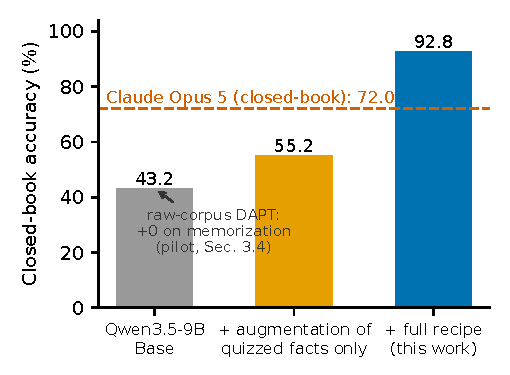
\includegraphics[width=\linewidth]{figures/fig1_ladder.pdf}
  \caption{\textbf{The recipe, not the corpus, carries the result.}
  Closed-book accuracy on the 125-question layered audit set. Continued
  pretraining on the raw 31M-token corpus leaves memorization at base level
  despite halving training loss (pilot measurement, \S\ref{sec:d4});
  augmenting only the quizzed facts helps only those facts (55.2\%); the full
  recipe (coverage of all facts, 24 diverse templates, reversed forms,
  whole-table narratives) reaches 92.8\%, surpassing Claude Opus~5 (dashed
  line).}
  \label{fig:ladder}
\end{figure}
